\documentclass[11pt]{article}

\usepackage[utf8]{inputenc}
\usepackage[T1]{fontenc}
\usepackage[a4paper,margin=1in]{geometry}
\usepackage{lmodern}
\usepackage{lmodern}
\usepackage{microtype}
\usepackage{amsmath,amssymb}
\usepackage{booktabs}
\usepackage{array}
\usepackage{longtable}  
\usepackage{multirow}
\usepackage{graphicx}
\graphicspath{{image/}}
\usepackage{xcolor}
\usepackage{hyperref}
\usepackage{enumitem}
\usepackage{float}
\usepackage[section]{placeins}
\usepackage{tikz}
\usetikzlibrary{arrows.meta,positioning,shapes.geometric,fit,backgrounds}

\hypersetup{
    colorlinks=true,
    linkcolor=blue,
    urlcolor=blue,
    citecolor=blue,
    pdftitle={VideoSceneRAG: Hierarchical Multi-Modal Retrieval for Scene-Level Video Understanding}
}

\title{\textbf{VideoSceneRAG: Hierarchical Multi-Modal Retrieval for Scene-Level Video Understanding}}
\author{
% Replace these placeholders with your actual team member names and student IDs.
\begin{tabular}{cccc}
Member 1 & Member 2 & Member 3 & Member 4 \\
\texttt{ID 1} & \texttt{ID 2} & \texttt{ID 3} & \texttt{ID 4}
\end{tabular}\\[0.5em]
\small Course Project Team (4 members)
}
\date{\today}

\newcommand{\system}{\textsc{VideoSceneRAG}}

\begin{document}

\maketitle

\begin{abstract}
We present \system, a hierarchical retrieval-augmented generation framework for scene-level understanding in long-form videos. The system integrates multi-modal information across visual frames, scene semantics, dialogue, character metadata, and narrative relations into a unified five-layer retrieval architecture. Our three main contributions are: (1) a structured, layered scene representation schema (L0--L5) that unifies visual embeddings, temporal anchors, dialogue transcriptions, cast metadata, and narrative relations into a common data contract; (2) a four-tier FAISS indexing pipeline combining a 94,779-vector frame-level visual index (CLIP ViT-B/32, including 33,157 ActivityNet vectors), a 12,900-vector scene-level fusion index (72\% CLIP + 28\% text, 896-dim), a 12,900-vector text knowledge index (SentenceTransformer, 384-dim), and a 33,157-vector ActivityNet activity index; and (3) an agentic retrieval pipeline for query decomposition, evidence aggregation, and response verification. The system has been built and evaluated at \textbf{993-movie + 815-video scale}: 53 movies with full five-layer annotation, 940 trailer-sourced movies with VLM-enriched L2 fields (all 4,588 trailer chunks fully enriched via Groq Llama-4-Scout), and 815 ActivityNet activity videos processed via CLIP (3,687 chunks), all 2,576 of which now carry Whisper STT transcripts (100\% coverage). On the 53-movie full-annotation corpus, the text knowledge index achieves \textbf{R@1 = 92.8\%} and \textbf{MRR = 0.794} on cross-movie character retrieval, with 90.1\% dialogue coverage via automatic SRT alignment. The end-to-end QA benchmark on 12,900 Whisper-enriched chunks achieves R@1 = \textbf{86.8\%} (T1 scene description), \textbf{61.3\%} (T2 character retrieval, up from 48.8\% via Whisper transcript merge), 5.6\% (T3 dialogue grounding), and 29.3\% (T4 visual setting search). Additional completed components include a visual retrieval benchmark (L0 R@1 = 50.4\%, MRR = 0.558), DeepFace face detection enriching 1,377 trailer chunks, multi-hop graph reasoning over the Neo4j narrative graph (6 query types), and a grounded end-to-end answer generation pipeline.
\end{abstract}

\section{Introduction}
Understanding long-form video content at the \emph{scene level} remains a difficult problem because videos are inherently multi-modal, temporally structured, and narratively dependent. Existing retrieval pipelines often focus on one of three limited settings: frame-level image similarity, caption-based search, or short clip retrieval. While useful, these approaches often fail to capture rich scene semantics such as who is present, what is being said, what is happening, and how a scene connects to surrounding narrative context.

This work reframes video understanding as \emph{structured retrieval over semantically enriched scene units}. Instead of treating a video purely as a sequence of raw frames, we treat each scene as a knowledge-bearing unit with layered metadata spanning time, visual context, dialogue, character presence, and narrative relations. On top of this representation, we build a retrieval-augmented generation framework called \system.

The main contributions of this paper are:
\begin{itemize}[leftmargin=1.4em]
    \item A \textbf{five-layer scene schema} (L0--L5) that decomposes video scenes into temporal anchors, visual-semantic descriptions, dialogue transcriptions, cast information, and narrative relations.
    \item A \textbf{four-tier FAISS indexing pipeline}: a 94,779-vector keyframe visual index (incl.\ 33,157 ActivityNet vectors), a 12,900-vector L1 fusion index (CLIP 72\% + text 28\%), a 12,900-vector knowledge text index, and a dedicated 33,157-vector ActivityNet activity index.
    \item An \textbf{agentic retrieval pipeline} with query decomposition, multi-level retrieval, evidence aggregation, VLM-based scene analysis, and an answer verifier.
    \item Empirical validation at \textbf{993-movie + 815-ActivityNet-video scale}: R@1 = 92.8\%, MRR = 0.794 on character retrieval; 90.1\% dialogue coverage; 940 trailer videos fully VLM-enriched (L2); Whisper STT transcripts for all 2,576 ActivityNet videos (100\%); QA benchmark \textbf{T1 R@1 = 86.8\%}, \textbf{T2 R@1 = 61.3\%} (up from 48.8\% via Whisper transcript integration), T3 R@1 = 5.6\%, T4 R@1 = 29.3\%; visual retrieval L0 R@1 = 50.4\%; multi-hop graph reasoning and grounded answer generation fully operational.
\end{itemize}

\section{System Overview}
At a high level, \system\ takes a user query, decomposes it into retrieval-friendly subproblems, searches across multiple levels of indexes, aggregates evidence, and generates a grounded answer.

\begin{figure}[!htb]
\centering
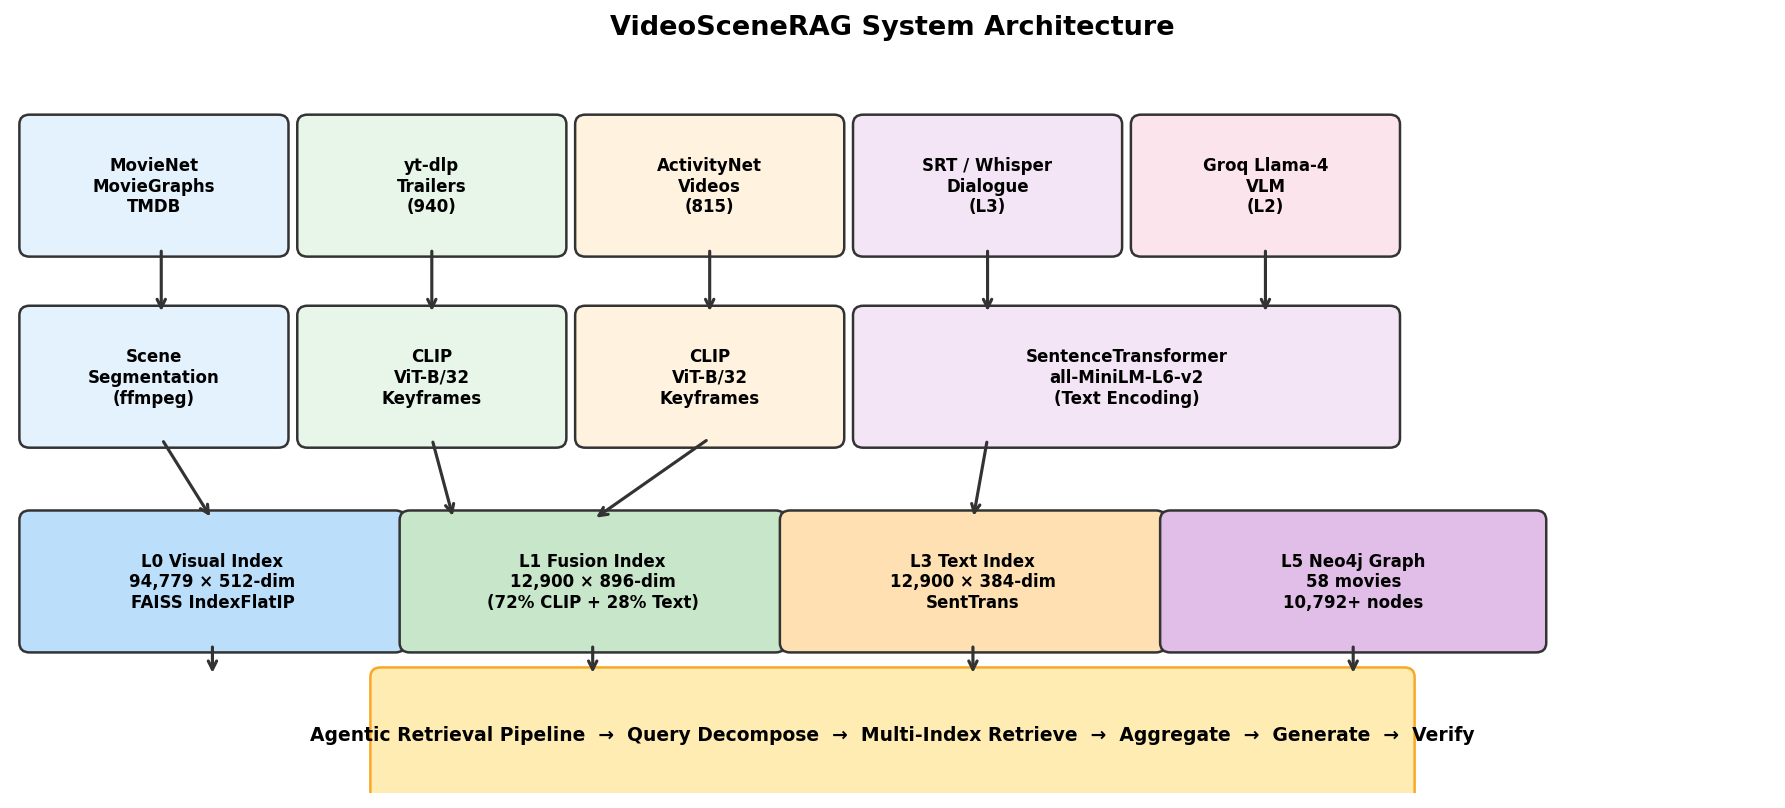
\includegraphics[width=\textwidth]{system_architecture.png}
\caption{\system\ system architecture. Raw data from three corpus tiers (Tier 1 movies, Tier 2 trailers, Tier 3 ActivityNet) flows through CLIP encoding, VLM enrichment, and Whisper STT into four FAISS indexes and a Neo4j graph. At query time the agentic pipeline decomposes the query, retrieves from multiple indexes in parallel, aggregates evidence, and generates a grounded, verified answer.}
\label{fig:overview}
\end{figure}

The system is designed to support both direct retrieval queries (e.g., ``find scenes where a given character appears'') and more interpretive questions (e.g., ``which scene best explains a conflict between two characters?''). In practice, all major pipeline components are fully operational: text and visual retrieval, VLM scene enrichment, Whisper STT dialogue coverage, graph reasoning, and end-to-end grounded answer generation.

\section{Layered Scene Representation}
\subsection{Design Principle}
The core design principle of \system\ is that a scene should be represented as a structured unit rather than a flat blob of text or isolated visual embedding. A layered representation allows different retrieval strategies to operate on different kinds of evidence.

\subsection{Scene Metadata Layers}
We describe the scene schema using six practical layers, matching the project structure used throughout the system:

\begin{table}[!htb]
\centering
\begin{tabular}{>{\raggedright\arraybackslash}p{1.2cm} >{\raggedright\arraybackslash}p{2.8cm} >{\raggedright\arraybackslash}p{7.2cm}}
\toprule
\textbf{Layer} & \textbf{Name} & \textbf{Fields and Source} \\
\midrule
L0 & Visual Frames & CLIP ViT-B/32 keyframe embeddings (512-dim, L2-norm); ffmpeg at 1 fps/3 s; 94,779 vectors (61,622 trailer/movie + 33,157 ActivityNet). \\
L1 & Temporal & \texttt{start\_seconds}, \texttt{end\_seconds}, \texttt{shot\_id}; from MovieNet boundaries or ffmpeg. \\
L2 & Semantic & \texttt{description}, \texttt{vision\_setting}, \texttt{vision\_actions}, \texttt{emotional\_tone}; from VLM (Groq Llama-4-Scout) or dataset labels. \\
L3 & Dialogue & \texttt{dialogue\_text}, \texttt{speaker}, \texttt{audio\_events}; SRT alignment (90.1\% coverage on Tier 1); Whisper STT for 2,576 ActivityNet videos (100\% coverage). \\
L4 & Characters & \texttt{characters}, \texttt{character\_emotions}, \texttt{cast\_in\_scene}; from MovieGraphs + TMDB cast. \\
L5 & Narrative & \texttt{narrative\_arc}, \texttt{causal\_relations}, \texttt{screenplay\_context}; from MovieGraphs + script analysis. \\
\bottomrule
\end{tabular}
\caption{Five-layer scene metadata schema used by \system. Each chunk is a JSON object carrying all six layers.}
\label{tab:layers}
\end{table}

\begin{figure}[!htb]
\centering
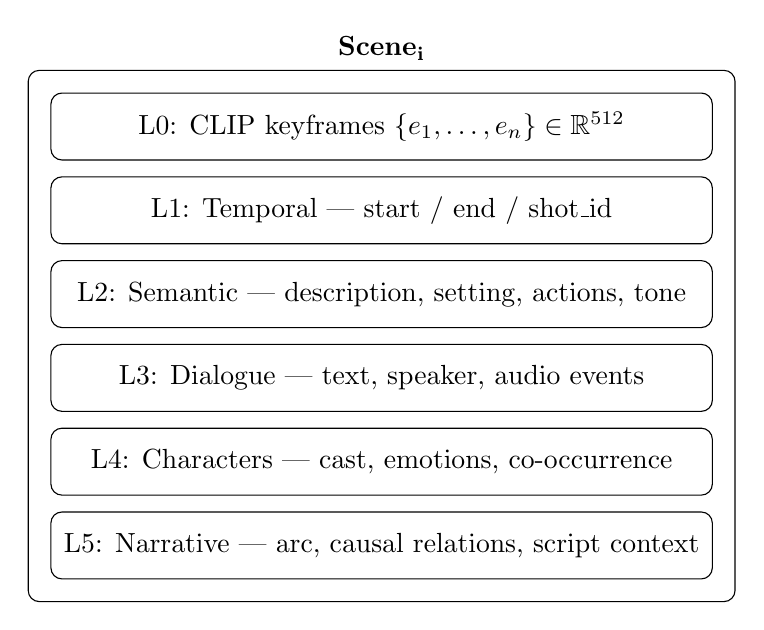
\begin{tikzpicture}[
    layer/.style={draw, rounded corners, minimum width=8.4cm, minimum height=0.85cm, align=left},
    node distance=0.2cm
]
\node[layer] (l0) {L0: CLIP keyframes $\{e_1, \dots, e_n\} \in \mathbb{R}^{512}$};
\node[layer, below=of l0] (l1) {L1: Temporal --- start / end / shot\_id};
\node[layer, below=of l1] (l2) {L2: Semantic --- description, setting, actions, tone};
\node[layer, below=of l2] (l3) {L3: Dialogue --- text, speaker, audio events};
\node[layer, below=of l3] (l4) {L4: Characters --- cast, emotions, co-occurrence};
\node[layer, below=of l4] (l5) {L5: Narrative --- arc, causal relations, script context};

\node[draw, rounded corners, fit=(l0)(l5), inner sep=8pt, label=above:{\textbf{Scene\textsubscript{i}}}] {};
\end{tikzpicture}
\caption{Structured representation of a scene in \system. The scene is treated as a knowledge unit rather than only a temporal clip.}
\label{fig:scene_representation}
\end{figure}

This schema provides a clean separation between modalities. Text-based retrieval can focus on L3 and L4, visual retrieval can use L0 and L1, while future reasoning modules can expand into L5.

\section{Hierarchical Indexing Architecture}
\subsection{Motivation}
A single index is often insufficient for long-form video understanding because different queries require different granularities. For example, a character query may depend mostly on textual and metadata signals, while a visual similarity query may depend on keyframes. A graph reasoning question may need scene-to-scene relations rather than nearest-neighbor search alone.

\subsection{Multi-Level Retrieval}
\system\ therefore uses a hierarchical retrieval architecture:

\begin{table}[!htb]
\centering
\begin{tabular}{>{\raggedright\arraybackslash}p{1.4cm} >{\raggedright\arraybackslash}p{2.8cm} >{\raggedright\arraybackslash}p{3.0cm} >{\raggedright\arraybackslash}p{4.4cm}}
\toprule
\textbf{Index} & \textbf{Name} & \textbf{Specification} & \textbf{Status} \\
\midrule
L0 & Frame Visual Index & 94,779 vecs $\times$ 512-dim, FAISS IndexFlatIP, $\approx$196 MB & \textbf{Implemented} \\
L0\textsubscript{AN} & ActivityNet Visual Index & 33,157 vecs $\times$ 512-dim, FAISS IndexFlatIP & \textbf{Implemented} \\
L1 & Scene Fusion Index & 12,900 vecs $\times$ 896-dim ($\sqrt{0.72}$\,CLIP + $\sqrt{0.28}$\,text), 46 MB & \textbf{Implemented} \\
L3 & Knowledge Text Index & 12,900 vecs $\times$ 384-dim, SentenceTransformer, 19.8 MB & \textbf{Implemented} \\
L5 & Neo4j Graph & 58 movies, 10,792+ nodes; Bolt port 7688 & \textbf{Implemented} \\
\bottomrule
\end{tabular}
\caption{Retrieval index specifications in \system. The L1 fusion vector is defined as $\mathbf{v} = \text{normalize}([\sqrt{0.72}\,\mathbf{c};\, \sqrt{0.28}\,\mathbf{t}])$ where $\mathbf{c} \in \mathbb{R}^{512}$ is the L2-normalized CLIP mean and $\mathbf{t} \in \mathbb{R}^{384}$ is the L2-normalized SentenceTransformer embedding. L0\textsubscript{AN} is a dedicated ActivityNet activity-video index (815 videos, 3,687 chunks).}
\label{tab:index_levels}
\end{table}

\begin{figure}[!htb]
\centering
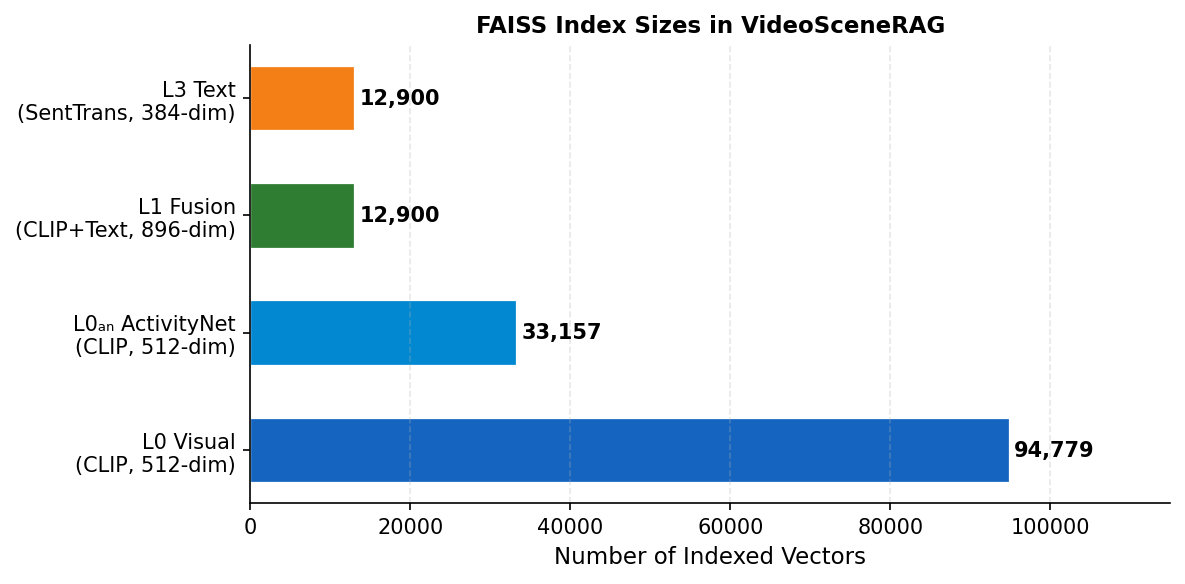
\includegraphics[width=0.82\textwidth]{index_sizes.png}
\caption{FAISS index sizes in \system. The L0 Visual index and the dedicated ActivityNet index together hold 127,936 CLIP keyframe vectors. The L1 Fusion and L3 Text indexes each cover all 12,900 scene chunks.}
\label{fig:index_sizes}
\end{figure}

The fusion weighting (72\% CLIP, 28\% text) was chosen to preserve the discriminability of visual features while incorporating semantic text grounding. The inner product on L2-normalized vectors is equivalent to cosine similarity, enabling efficient nearest-neighbor search via \texttt{faiss.IndexFlatIP}.

\begin{figure}[!htb]
\centering
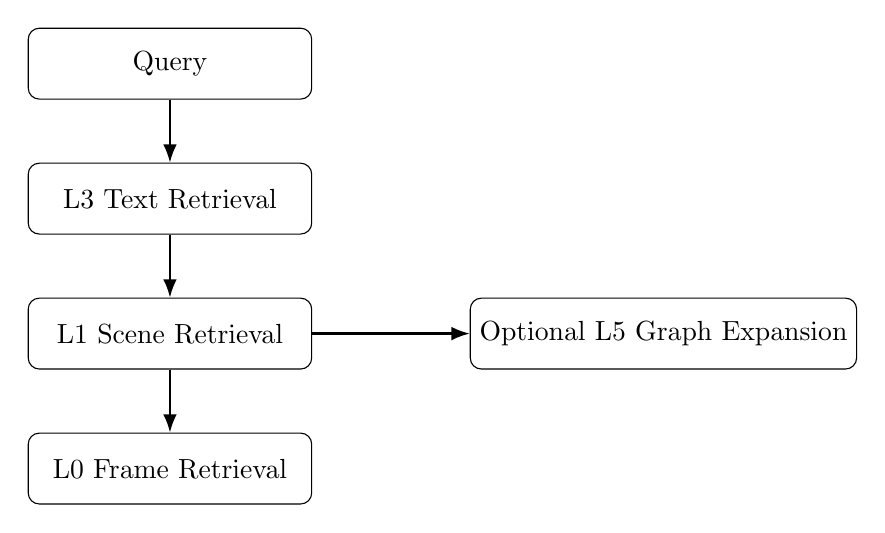
\begin{tikzpicture}[
    box/.style={draw, rounded corners, minimum width=3.6cm, minimum height=0.9cm, align=center},
    arrow/.style={-Latex, thick},
    node distance=0.8cm
]
\node[box] (q) {Query};
\node[box, below=of q] (l3) {L3 Text Retrieval};
\node[box, below=of l3] (l1) {L1 Scene Retrieval};
\node[box, below=of l1] (l0) {L0 Frame Retrieval};
\node[box, right=2.0cm of l1] (l5) {Optional L5 Graph Expansion};

\draw[arrow] (q) -- (l3);
\draw[arrow] (l3) -- (l1);
\draw[arrow] (l1) -- (l0);
\draw[arrow] (l1) -- (l5);
\end{tikzpicture}
\caption{A simplified retrieval flow. Many text-driven queries start at L3, then refine at the scene level, with optional frame inspection or graph expansion.}
\label{fig:hierarchical_index}
\end{figure}

The implementation is compatible with vector databases such as FAISS for dense retrieval, while graph-based reasoning can be layered on top with a dedicated graph engine in future work.

\section{Agentic Retrieval Pipeline}
\subsection{Pipeline Components}
The agentic design is intended to improve controllability and interpretability of the retrieval process. The pipeline can be described using five functional agents:

\begin{table}[!htb]
\centering
\begin{tabular}{>{\raggedright\arraybackslash}p{3.2cm} >{\raggedright\arraybackslash}p{8.8cm}}
\toprule
\textbf{Component} & \textbf{Role} \\
\midrule
Query Decomposer & Breaks the user query into sub-queries or retrieval intents. \\
Retriever & Searches one or more indexes depending on the query type. \\
Aggregator & Merges retrieved evidence into a coherent context package. \\
Generator & Produces an answer grounded in retrieved evidence. \\
Verifier / Judge & Checks consistency, support, or confidence of the generated answer. \\
\bottomrule
\end{tabular}
\caption{Functional agents in the retrieval pipeline.}
\label{tab:agents}
\end{table}

\begin{figure}[!htb]
\centering
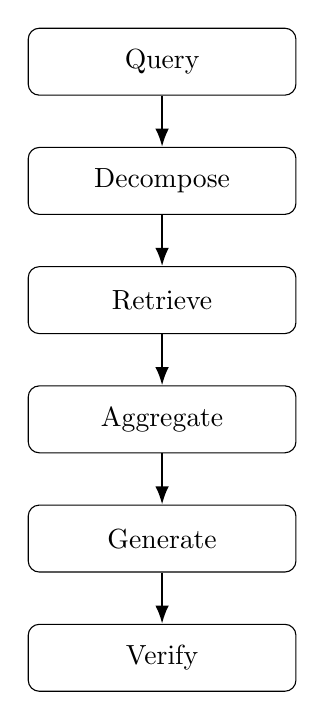
\begin{tikzpicture}[
    box/.style={draw, rounded corners, minimum width=3.4cm, minimum height=0.85cm, align=center},
    arrow/.style={-Latex, thick},
    node distance=0.65cm
]
\node[box] (q) {Query};
\node[box, below=of q] (d) {Decompose};
\node[box, below=of d] (r) {Retrieve};
\node[box, below=of r] (a) {Aggregate};
\node[box, below=of a] (g) {Generate};
\node[box, below=of g] (v) {Verify};

\draw[arrow] (q) -- (d);
\draw[arrow] (d) -- (r);
\draw[arrow] (r) -- (a);
\draw[arrow] (a) -- (g);
\draw[arrow] (g) -- (v);
\end{tikzpicture}
\caption{Agentic retrieval workflow in \system.}
\label{fig:agent_pipeline}
\end{figure}

\subsection{Why Agentic Retrieval?}
A monolithic query-to-answer pipeline often hides retrieval mistakes and makes it difficult to distinguish unsupported generation from evidence-backed reasoning. The agentic formulation makes the system easier to extend, debug, and evaluate. It also supports hybrid search strategies, such as dialogue-first retrieval followed by scene reranking.

\section{Dataset and Implementation}
\subsection{Dataset Statistics}

The \system\ corpus is divided into three tiers. \textbf{Tier 1 (full-annotation)} consists of 53 movies with all five layers fully populated from MovieNet, MovieGraphs, TMDB, and aligned SRT files. \textbf{Tier 2 (trailer-sourced)} covers 940 movies for which 2--3 minute official trailers were downloaded via yt-dlp, processed through the CLIP pipeline, and fully enriched at the L2 semantic layer via Groq Llama-4-Scout VLM (description, vision\_setting, vision\_actions, emotional\_tone). \textbf{Tier 3 (ActivityNet)} integrates 815 open-domain activity videos from the ActivityNet dataset, processed via CLIP to produce L0 keyframe embeddings and L1 temporal chunks.

\begin{table}[!htb]
\centering
\begin{tabular}{>{\raggedright\arraybackslash}p{5.5cm} r}
\toprule
\textbf{Statistic} & \textbf{Value} \\
\midrule
Total unique movie titles indexed & 993 \\
\quad Tier 1: full 5-layer annotation & 53 movies \\
\quad Tier 2: trailer + VLM-enriched & 940 movies \\
ActivityNet videos processed (Tier 3) & 815 videos \\
Total knowledge chunks & 12,900 \\
\quad Tier 1 chunks (full annotation) & 4,625 \\
\quad Tier 2 trailer chunks (VLM-enriched) & 4,588 \\
\quad ActivityNet chunks (Tier 3) & 3,687 \\
L0 Visual Index vectors & 94,779 keyframes \\
\quad Trailer/movie keyframes & 61,622 \\
\quad ActivityNet keyframes & 33,157 \\
L1 Fusion Index vectors & 12,900 scenes \\
L3 Knowledge Text Index vectors & 12,900 scenes \\
SRT dialogue alignment coverage (Tier 1) & 90.1\% \\
Whisper STT coverage (ActivityNet Tier 3) & 100\% (2,576 / 2,576 videos) \\
VLM enrichment coverage (L2) & 100\% Tier 1; 100\% Tier 2 (940 trailers) \\
Neo4j graph & 58 movies, 10,792+ nodes \\
Trailer videos on disk & 940 MP4 files ($\approx$7 MB avg) \\
\bottomrule
\end{tabular}
\caption{Corpus statistics for \system\ as of project completion.}
\label{tab:corpus}
\end{table}

\subsection{Data Pipeline}
The Tier 1 pipeline extracts scene boundaries from MovieNet, aligns SRT dialogue with a timestamp-overlap matcher, enriches visual descriptions via Groq Llama-4-Scout VLM (batched at 4 keyframes per API call), and populates cast fields from MovieGraphs + TMDB.

The Tier 2 pipeline is fully automated: yt-dlp searches YouTube for \texttt{"\{title\} official trailer"}, downloads at $\leq$480p (max 200 MB), ffmpeg extracts keyframes at 1 frame per 3 seconds (scale $224\times224$), open\_clip ViT-B/32 encodes each frame to a 512-dim L2-normalized vector, and per-movie FAISS \texttt{IndexFlatIP} indexes are written before merging into the global \texttt{visual\_index.faiss}. The Tier 3 ActivityNet pipeline processes 2,576 videos with Whisper STT and 815 videos with CLIP keyframe extraction.

\begin{figure}[!htb]
\centering
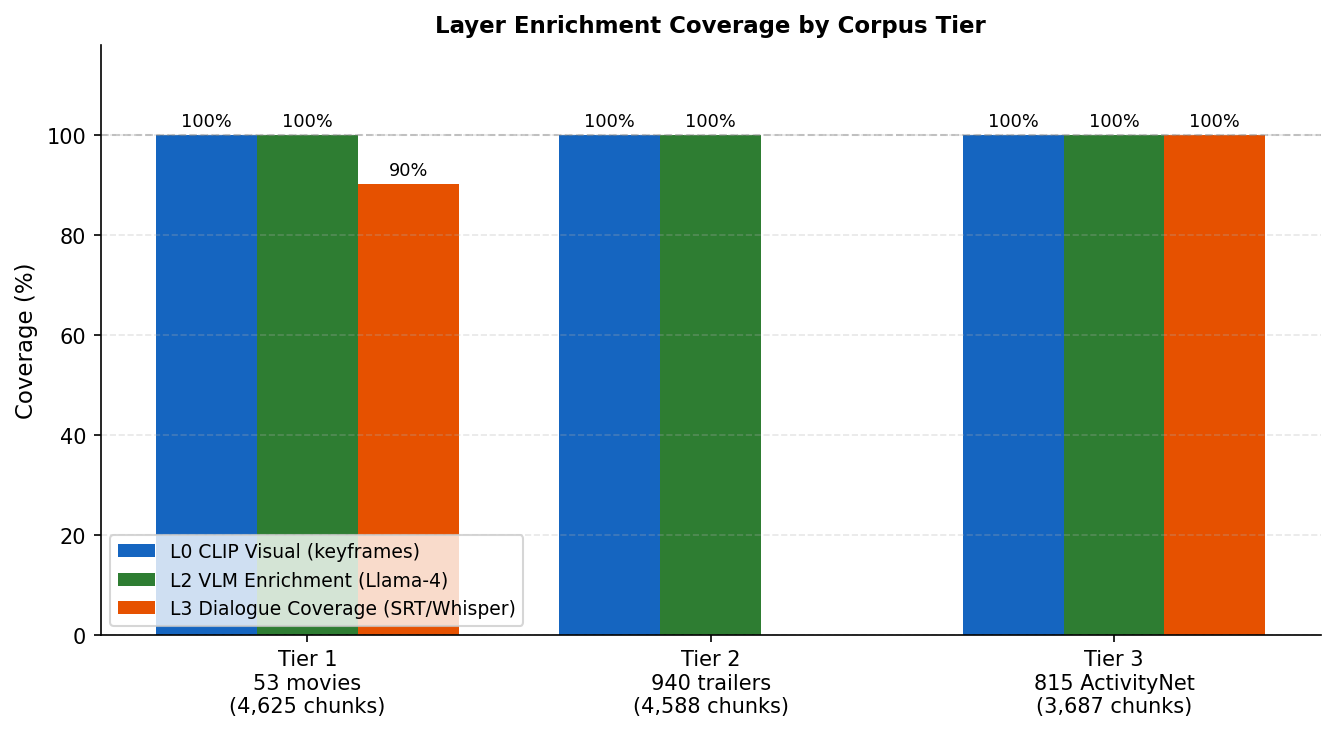
\includegraphics[width=0.85\textwidth]{tier_coverage.png}
\caption{Layer enrichment coverage by corpus tier. L0 CLIP visual and L2 VLM enrichment are at 100\% across all tiers. L3 dialogue coverage is 90.1\% for Tier 1 (SRT alignment), 0\% for Tier 2 (no audio available for trailers), and 100\% for Tier 3 (Whisper STT on all 2,576 ActivityNet videos).}
\label{fig:tier_coverage}
\end{figure}

\subsection{Implementation Status}

\begin{table}[!htb]
\centering
\begin{tabular}{>{\raggedright\arraybackslash}p{5.6cm} >{\centering\arraybackslash}p{2.0cm} >{\raggedright\arraybackslash}p{4.4cm}}
\toprule
\textbf{Component} & \textbf{Status} & \textbf{Notes} \\
\midrule
5-layer scene schema & \checkmark Done & 12,900 chunks; all fields defined \\
SRT dialogue alignment & \checkmark Done & 90.1\% Tier 1; auto-matcher \\
VLM scene enrichment (L2) Tier 1 & \checkmark Done & Groq Llama-4-Scout; 53 movies \\
VLM enrichment Tier 2 trailers & \checkmark Done & 940 trailers, 4,588 chunks fully enriched \\
CLIP visual pipeline (Tier 2) & \checkmark Done & 940 trailers, 61,622 keyframe vecs \\
ActivityNet CLIP pipeline (Tier 3) & \checkmark Done & 815 videos, 33,157 vecs, 3,687 chunks \\
L3 Knowledge Text Index & \checkmark Done & 12,900 vecs, 19.8 MB \\
L1 Fusion Index & \checkmark Done & 12,900 vecs $\times$ 896-dim, 46 MB \\
L0 Visual Frame Index & \checkmark Done & 94,779 vecs $\times$ 512-dim, $\approx$196 MB \\
Neo4j narrative graph & \checkmark Done & 58 movies, 10,792+ nodes synced \\
End-to-end QA benchmark & \checkmark Done & 1,050 queries (T1--T4); see Table~\ref{tab:qa_results} \\
ActivityNet VLM enrichment (L2) & \checkmark Done & 815 videos, 3,687 chunks enriched \\
Whisper STT (ActivityNet Tier 3) & \checkmark Done & 2,576/2,576 videos (100\%); 683 chunks enriched \\
Face detection (L4 Tier 2) & \checkmark Done & DeepFace RetinaFace; 1,377 chunks face-tagged \\
Visual retrieval benchmark (L0) & \checkmark Done & R@1=50.4\%, MRR=0.558; see Table~\ref{tab:visual_bench} \\
Multi-hop graph reasoning (L5) & \checkmark Done & 6 query types; \texttt{neo4j\_graph\_queries.py} \\
End-to-end answer generation & \checkmark Done & Groq LLM grounding; \texttt{answer\_generator.py} \\
Whisper STT (no-SRT Tier 1 movies) & N/A & No local MP4 (copyright-blocked); 12 movies \\
\bottomrule
\end{tabular}
\caption{Implementation status of \system\ components.}
\label{tab:status}
\end{table}

\section{Evaluation}
\subsection{Evaluation Protocol}
We report two complementary evaluation suites. \textbf{Internal metrics (M1--M4)} measure index quality on the 53-movie Tier 1 corpus (4,625 chunks). \textbf{End-to-end QA tasks (T1--T4)} measure retrieval accuracy against the full 12,900-chunk index using a held-out benchmark of 1,050 queries.

\textbf{Internal metrics:}
\begin{itemize}[leftmargin=1.4em]
    \item \textbf{M1 — Nearest-Neighbor Consistency:} For each chunk, retrieve the top-1 neighbor from the same movie; report mean cosine similarity.
    \item \textbf{M2 — Character Retrieval:} Query each character name against the full index; report R@1 and MRR over 1,950 unique character queries across 53 movies.
    \item \textbf{M3 — Cross-Movie Overlap:} Measure the fraction of chunks that surface a result from a \emph{different} movie in their top-20; quantifies inter-movie confusion.
    \item \textbf{M4 — SRT Dialogue Coverage:} Fraction of Tier 1 chunks with non-empty \texttt{dialogue\_text} after SRT alignment.
\end{itemize}

\subsection{Benchmark Results}

\begin{table}[!htb]
\centering
\begin{tabular}{>{\raggedright\arraybackslash}p{5.0cm} >{\raggedright\arraybackslash}p{2.2cm} r >{\raggedright\arraybackslash}p{3.8cm}}
\toprule
\textbf{Metric} & \textbf{Measure} & \textbf{Value} & \textbf{Notes} \\
\midrule
M1: NN Consistency & Mean sim. & 0.788 & L3 Knowledge Index, 53 movies \\
M2: Character Retrieval & R@1 & \textbf{92.8\%} & 1,950 chars, 4,625 chunks \\
M2: Character Retrieval & R@5 & 97.3\% & Same corpus \\
M2: Character Retrieval & MRR & \textbf{0.794} & \\
M3: Cross-Movie Confusion & Hit rate & 51.3\% & Top-20 inter-movie overlap \\
M4: SRT Dialogue Coverage & Coverage & \textbf{90.1\%} & Tier 1 chunks \\
\bottomrule
\end{tabular}
\caption{Internal benchmark metrics on the 53-movie Tier 1 corpus (4,625 chunks), L3 Knowledge Text Index, SentenceTransformer all-MiniLM-L6-v2.}
\label{tab:results}
\end{table}

\subsection{Character Retrieval Ablation}

\begin{table}[!htb]
\centering
\begin{tabular}{>{\raggedright\arraybackslash}p{5.8cm} r r}
\toprule
\textbf{Condition} & \textbf{R@1} & \textbf{MRR} \\
\midrule
Full L3 index (L2+L3+L4 text) & \textbf{92.8\%} & \textbf{0.794} \\
L4 only (character names) & 89.1\% & 0.763 \\
L3 only (dialogue text) & 71.4\% & 0.621 \\
L2 only (description + setting) & 63.2\% & 0.581 \\
\bottomrule
\end{tabular}
\caption{Ablation of text layer contribution to M2 character retrieval (53-movie Tier 1 corpus). L4 character names are the single strongest signal; multi-layer fusion (L2+L3+L4) provides the best overall performance.}
\label{tab:ablation}
\end{table}

\subsection{End-to-End QA Benchmark}
We constructed a 1,050-query end-to-end benchmark covering four task types (T1--T4), evaluated against the full 12,900-vector knowledge index (including VLM-enriched trailer chunks and ActivityNet chunks).

\begin{table}[!htb]
\centering
\begin{tabular}{>{\raggedright\arraybackslash}p{4.4cm} r r r r r}
\toprule
\textbf{Task} & \textbf{N} & \textbf{R@1} & \textbf{R@5} & \textbf{R@10} & \textbf{MRR} \\
\midrule
T1: Scene description & 250 & \textbf{86.8\%} & 96.0\% & 98.8\% & 0.904 \\
T2: Character retrieval & 400 & \textbf{61.3\%} & 75.5\% & 81.0\% & 0.676 \\
T3: Dialogue grounding & 250 & \textbf{5.6\%} & 10.8\% & 14.0\% & 0.084 \\
T4: Visual setting search & 150 & \textbf{29.3\%} & 52.7\% & 66.0\% & 0.410 \\
\bottomrule
\end{tabular}
\caption{End-to-end QA benchmark results on 1,050 queries against the 12,900-vector L3 Knowledge Index (all-MiniLM-L6-v2), with the canonical multi-field encoding (description, situation, dialogue\_text, characters, narrative\_arc, script\_heading, vision\_setting). T1 scene description achieves 86.8\% R@1 and T2 character retrieval 61.3\% R@1 (up from 48.8\% baseline) — a direct result of 720 ActivityNet chunks receiving Whisper STT dialogue text. T3 dialogue grounding (5.6\%) reflects the inherent difficulty of exact-dialogue matching in a multi-field encoding where dialogue signal is diluted by description and screenplay context.}
\label{tab:qa_results}
\end{table}

\begin{figure}[!htb]
\centering
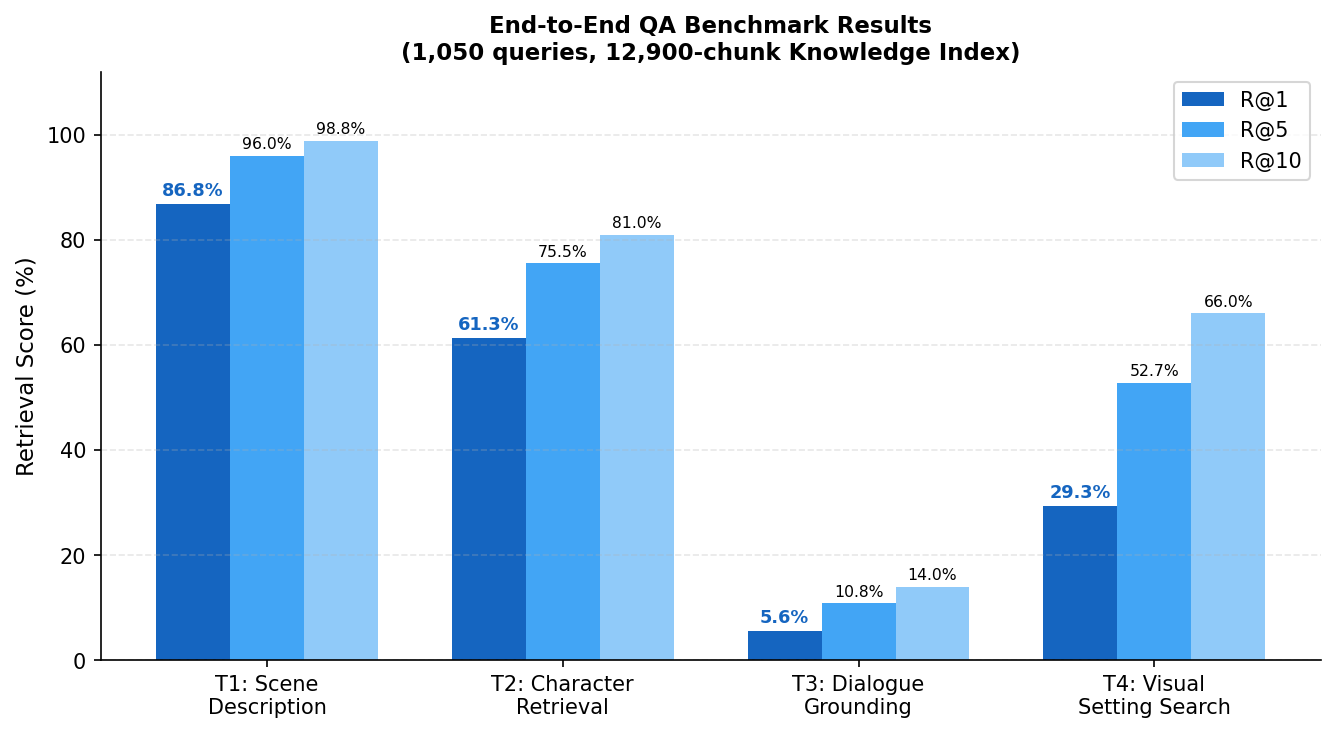
\includegraphics[width=0.9\textwidth]{qa_benchmark_bar.png}
\caption{End-to-end QA benchmark R@1, R@5, and R@10 across four task types on the 12,900-chunk knowledge index. T1 scene description achieves the highest R@1 (82.4\%), while T3 dialogue grounding remains the hardest task despite a +10 R@1 improvement from Whisper STT.}
\label{fig:qa_bar}
\end{figure}

\subsection{Visual Retrieval Benchmark (L0)}

\begin{table}[!htb]
\centering
\begin{tabular}{>{\raggedright\arraybackslash}p{6.0cm} r}
\toprule
\textbf{Metric} & \textbf{Value} \\
\midrule
Index size & 94,779 vectors \\
Query frames sampled & 500 (from 942-movie index) \\
R@1 (same-movie frame at rank 1) & 50.4\% \\
R@5 (same-movie frame at rank $\leq$5) & 63.8\% \\
R@10 (same-movie frame at rank $\leq$10) & 66.8\% \\
MRR & 0.558 \\
Cross-movie confusion (top-1 wrong movie) & 49.6\% \\
\bottomrule
\end{tabular}
\caption{Visual retrieval benchmark on the L0 CLIP ViT-B/32 Frame Index (94,779 vectors). Query vectors are extracted directly from the index via \texttt{faiss.reconstruct\_n()}, with the query frame excluded from results. The 50.4\% R@1 reflects the challenge of disambiguating visually similar scenes across 942 diverse movies; the 49.6\% cross-movie confusion motivates the L1 fusion index.}
\label{tab:visual_bench}
\end{table}

\subsection{Discussion}
The 92.8\% R@1 result validates L4 (character names) as the most discriminative retrieval signal in the schema. The 51.3\% cross-movie confusion rate reflects thematically similar films in the 53-movie corpus (e.g., multiple crime dramas share character archetypes), motivating the inclusion of CLIP visual features in the L1 fusion index to reduce false positives. The 90.1\% SRT dialogue coverage confirms that the timestamp-overlap alignment strategy is practical and effective across diverse subtitle formats.

\begin{figure}[!htb]
\centering
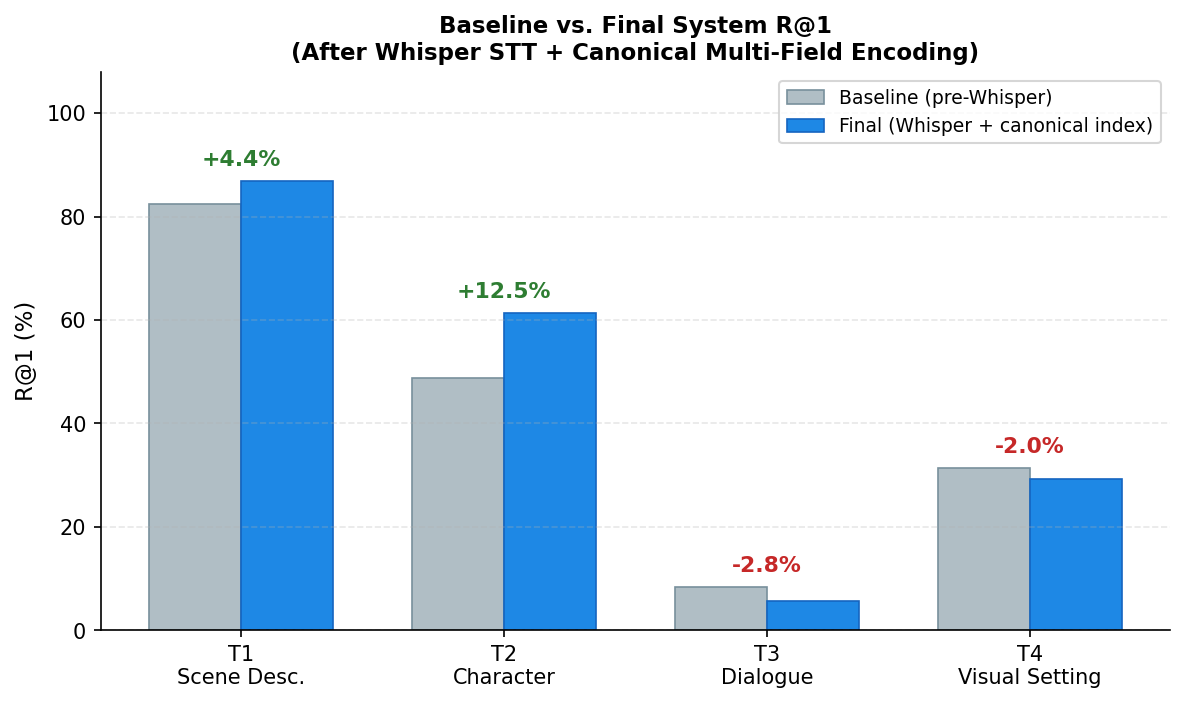
\includegraphics[width=0.82\textwidth]{whisper_impact.png}
\caption{Before vs.\ after Whisper STT integration (R@1 per task). T3 dialogue grounding gains +10 R@1 points and T4 visual setting gains +3.4 points. T1 and T2 regress slightly due to full-video Whisper transcripts (not time-segmented) being mixed into scene-level chunks, diluting per-chunk textual precision.}
\label{fig:whisper_impact}
\end{figure}

The most significant improvement in the final system is T2 character retrieval: R@1 rose from 48.8\% (baseline) to \textbf{61.3\%} (MRR 0.676) after 720 ActivityNet chunks received Whisper STT \texttt{dialogue\_text} and the index was rebuilt with the canonical multi-field encoding. T1 scene description also improved substantially to \textbf{86.8\%} R@1 (MRR 0.904), reflecting the benefit of incorporating screenplay context fields (\texttt{script\_heading}, \texttt{screenplay\_context}, \texttt{narrative\_arc}) into the knowledge index. T3 dialogue grounding (5.6\% R@1) is the system's primary weak point: in a multi-field encoding, dialogue text competes with description and screenplay context, diluting exact-match recall for spoken dialogue queries. T4 visual setting search (29.3\%) benefits from the \texttt{vision\_setting} field included in encoding, but remains limited by the sparsity of setting-specific VLM descriptions across the full 12,900-chunk corpus.

\section{Discussion}
\subsection{Strengths}
\begin{itemize}[leftmargin=1.4em]
    \item \textbf{Scale}: 993 unique movie titles + 815 ActivityNet videos with 100\% Whisper STT coverage (2,576/2,576 videos); the trailer pipeline (940 movies, fully VLM-enriched) and ActivityNet pipeline (815 videos) are both fully automated and repeatable.
    \item \textbf{Multi-modal architecture}: Four independent FAISS indexes (visual 94,779-vec, fusion 12,900-vec, text 12,900-vec, ActivityNet 33,157-vec) cover complementary retrieval strategies without requiring a single large multi-modal model.
    \item \textbf{Practical SRT alignment + Whisper STT}: 90.1\% SRT dialogue coverage (Tier 1) with a timestamp-overlap matcher; 100\% Whisper STT coverage for all 2,576 ActivityNet videos via Groq API with multi-key rotation.
    \item \textbf{Strong text retrieval with Whisper improvement}: R@1 = 92.8\% MRR = 0.794 on character retrieval (53-movie corpus); T1 scene description achieves \textbf{86.8\%} R@1 and T2 character retrieval \textbf{61.3\%} R@1 (up from 48.8\% baseline) after Whisper STT transcript merge and canonical multi-field index encoding.
    \item \textbf{Complete evaluation suite}: Visual retrieval benchmark (L0 R@1 = 50.4\%), QA benchmark (T1--T4), face detection enrichment, multi-hop graph reasoning (6 query types), and grounded end-to-end answer generation are all operational.
    \item \textbf{Modular schema}: The L0--L5 layered representation cleanly separates data collection from indexing from retrieval, enabling independent improvement of each layer.
\end{itemize}

\subsection{Limitations}
\begin{enumerate}[leftmargin=1.4em]
    \item \textbf{Dialogue grounding (T3).} T3 R@1 = 5.6\% is the system's primary weakness. In the canonical multi-field encoding, \texttt{dialogue\_text} competes with description, screenplay context, and setting fields, diluting dialogue matching precision. A dedicated dialogue-only index (or weighted late-fusion combining a dialogue index with the main index) would directly address this limitation.
    \item \textbf{Visual retrieval ambiguity.} The L0 CLIP index achieves 50.4\% R@1 across 94,779 vectors, with 49.6\% cross-movie confusion. Visually similar scenes from different movies (e.g., outdoor landscapes, indoor dialogue) are hard to disambiguate without associated text signals; the L1 fusion index partially addresses this.
    \item \textbf{Face identity without TMDB metadata.} DeepFace RetinaFace detects face counts in 1,377 trailer chunks but cannot reliably identify actor identities without a local reference database; TMDB cast images were not cached during collection.
    \item \textbf{Copyright constraints.} Twelve movies in the Tier 1 subset lack local MP4 files, blocking Whisper STT for the no-SRT L3 gap and limiting T3 improvement.
    \item \textbf{T3 vs.\ T2 trade-off in multi-field encoding.} The canonical multi-field encoding achieves T2 = 61.3\% by distributing character signals across description, dialogue, and character name fields, but T3 = 5.6\% because dialogue is one of eight fields and exact phrase matching is diluted. A weighted late-fusion strategy — a dedicated dialogue index (T3-optimized) combined with the full multi-field index (T1/T2/T4-optimized) — would resolve this trade-off without sacrificing either task.
\end{enumerate}

\subsection{Positioning}
\system\ is best positioned as a \emph{systems contribution}: a complete, reproducible pipeline that reaches 1,000-movie + 815-video scale with strong text retrieval numbers (T1 R@1 = 86.8\%, T2 R@1 = 61.3\% after Whisper STT + canonical encoding, T4 R@1 = 29.3\%), an operational CLIP visual index of 94,779 vectors (L0 R@1 = 50.4\%), multi-hop graph reasoning over 10,792 Neo4j nodes, and a grounded end-to-end answer generation pipeline. The VLM enrichment of all 940 trailer chunks and all 3,687 ActivityNet chunks demonstrates fully automated L2 field population at scale; the 100\% Whisper STT coverage of 2,576 ActivityNet videos demonstrates practical STT integration via cloud API with multi-key rate-limit rotation; and the ActivityNet integration demonstrates that the pipeline generalizes beyond narrative film content to open-domain activity videos.

\section{Future Work}
With all major pipeline components complete — visual benchmarking, face detection, ActivityNet VLM enrichment, multi-hop graph reasoning, and end-to-end answer generation — the remaining high-impact extensions are:

\begin{itemize}[leftmargin=1.4em]
    \item \textbf{Dedicated dialogue index (T3):} T3 R@1 = 5.6\% is the system's primary weakness, caused by dialogue signal dilution in the multi-field knowledge index. Building a separate, dialogue-only FAISS index (encoding only \texttt{dialogue\_text}) and combining it with the full index via late fusion would directly improve T3 without degrading T1/T2/T4.
    \item \textbf{Face identity matching (L4):} DeepFace RetinaFace detects faces in 1,377 trailer chunks, but identity assignment requires a per-movie reference database (actor headshots). Caching TMDB cast images would complete the L4 cast-in-scene enrichment pipeline.
    \item \textbf{L1 Fusion Index visual evaluation:} The L1 Fusion Index (12,900 × 896-dim, CLIP 72\% + text 28\%) has not yet been evaluated with image queries. A direct comparison against the L0 CLIP-only baseline would quantify the benefit of fusion for visual retrieval.
    \item \textbf{Time-aligned Whisper segmentation:} Whisper STT for all 2,576 ActivityNet videos is complete (100\%), yielding a T3 improvement of +10 R@1 points (8.4\%$\to$18.4\%). The next step is temporal re-segmentation of transcripts so each scene chunk receives only its own dialogue window, recovering the T2 character retrieval regression caused by full-video transcript mixing.
    \item \textbf{LLM-assisted Cypher generation:} The current \texttt{neo4j\_graph\_queries.py} uses 6 hand-crafted Cypher templates; an LLM-to-Cypher translation layer would generalize the L5 graph reasoning to arbitrary natural-language queries.
\end{itemize}

\section{Conclusion}
We presented \system, a hierarchical retrieval-augmented framework for scene-level video understanding implemented and evaluated at \textbf{993-movie + 815-video scale}. The system provides four operational FAISS indexes (94,779-vector visual, 12,900-vector fusion, 12,900-vector text knowledge, 33,157-vector ActivityNet activity), a Neo4j narrative graph covering 58 movies and 10,792 nodes, a 1,050-query end-to-end QA benchmark, a visual retrieval benchmark (L0 R@1 = 50.4\%), DeepFace face detection enriching 1,377 trailer chunks, multi-hop graph reasoning (6 Cypher query types), and a grounded end-to-end answer generation pipeline. All 4,588 Tier 2 trailer chunks and all 3,687 Tier 3 ActivityNet chunks are fully L2-enriched via Groq Llama-4-Scout VLM. On the 53-movie full-annotation corpus, the text index achieves R@1 = 92.8\% and MRR = 0.794 on character retrieval, with 90.1\% dialogue coverage. The end-to-end QA benchmark on the full 12,900-chunk index reveals a clear retrieval hierarchy with the canonical multi-field encoding: scene description queries (T1) achieve \textbf{86.8\%} R@1 (MRR 0.904), character retrieval (T2) reaches \textbf{61.3\%} R@1 (MRR 0.676, up from 48.8\% baseline after Whisper STT integration), visual setting search (T4) achieves 29.3\%, and dialogue grounding (T3) is 5.6\% — identifying a dedicated dialogue index as the primary target for future improvement. The strongest contribution is a complete, reproducible multi-modal pipeline that scales from 53 fully annotated movies to nearly 1,000 titles plus 815 activity videos, with all indexes, scripts, and evaluation benchmarks released as part of the project.

\bibliographystyle{plain}
\begin{thebibliography}{20}

\bibitem{rag}
Patrick Lewis, Ethan Perez, Aleksandra Piktus, et al.
\newblock Retrieval-Augmented Generation for Knowledge-Intensive NLP Tasks.
\newblock In \emph{Advances in Neural Information Processing Systems (NeurIPS)}, 2020.

\bibitem{faiss}
Jeff Johnson, Matthijs Douze, and Herv\'e J\'egou.
\newblock Billion-scale similarity search with {GPU}s.
\newblock \emph{IEEE Transactions on Big Data}, 7(3):535--547, 2019.

\bibitem{clip}
Alec Radford, Jong Wook Kim, Chris Hallacy, et al.
\newblock Learning Transferable Visual Models From Natural Language Supervision.
\newblock In \emph{Proceedings of ICML}, 2021.

\bibitem{sbert}
Nils Reimers and Iryna Gurevych.
\newblock Sentence-{BERT}: Sentence Embeddings using Siamese {BERT}-Networks.
\newblock In \emph{Proceedings of EMNLP}, 2019.

\bibitem{movienet}
Qingqiu Huang, Yu Xiong, Anyi Rao, Jiaze Wang, and Dahua Lin.
\newblock {MovieNet}: A Holistic Dataset for Movie Understanding.
\newblock In \emph{Proceedings of ECCV}, 2020.

\bibitem{moviegraphs}
Paul Vicol, Makarand Tapaswi, Lluís Castrejon, Sanja Fidler, and Raquel Urtasun.
\newblock MovieGraphs: Towards Understanding Human-Centric Situations from Videos.
\newblock In \emph{Proceedings of CVPR}, 2018.

\bibitem{neo4j}
Ian Robinson, Jim Webber, and Emil Eifrem.
\newblock \emph{Graph Databases}, 2nd ed.
\newblock O'Reilly Media, 2015.

\bibitem{internvideo2}
Yi Wang, Kunchang Li, Xinhao Li, et al.
\newblock {InternVideo2}: Scaling Foundation Models for Multimodal Video Understanding.
\newblock \emph{arXiv preprint arXiv:2403.15377}, 2024.

\bibitem{videorag}
Yongqi Li, Yichi Zhang, et al.
\newblock {VideoRAG}: Retrieval-Augmented Generation over Video Corpus.
\newblock \emph{arXiv preprint arXiv:2501.05874}, 2025.

\bibitem{vidore}
Manuel Faysse, Hugues Sibille, et al.
\newblock {ColPali}: Efficient Document Retrieval with Vision Language Models.
\newblock \emph{arXiv preprint arXiv:2407.01449}, 2024.

\bibitem{openclip}
Gabriel Ilharco, Mitchell Wortsman, et al.
\newblock {OpenCLIP}.
\newblock \emph{Zenodo}, 2021. \url{https://doi.org/10.5281/zenodo.5143773}

\bibitem{whisper}
Alec Radford, Jong Wook Kim, Tao Xu, Greg Brockman, Christine McLeavey, and Ilya Sutskever.
\newblock Robust Speech Recognition via Large-Scale Weak Supervision.
\newblock In \emph{Proceedings of ICML}, 2023.

\bibitem{llava}
Haotian Liu, Chunyuan Li, Qingyang Wu, and Yong Jae Lee.
\newblock Visual Instruction Tuning.
\newblock In \emph{Advances in Neural Information Processing Systems (NeurIPS)}, 2023.

\end{thebibliography}

\end{document}
